%__________________________________PREAMBLE_________________________________%
\documentclass[12pt,english]{article}
\usepackage[a4paper, left = 2cm,%
            right=2cm,top=2cm,bottom=2cm,%
            footskip=.25in]{geometry}
\usepackage{amsfonts, amsmath, amssymb, physics}
\usepackage[utf8]{inputenc}
\usepackage[english]{babel}
\usepackage[backend=biber, citestyle=nature]{biblatex}
\usepackage[nottoc]{tocbibind}
\usepackage{indentfirst, halloweenmath, calligra, %
            esint, graphicx, hyperref, xcolor, float}
\hypersetup{
  colorlinks   = true, %Colours links instead of ugly boxes
  urlcolor     = blue, %Colour for external hyperlinks
  linkcolor    = blue, %Colour of internal links
  citecolor   = red %Colour of citations
}
\graphicspath{{./images/}}
%__________________________________COMMANDS_________________________________%
\addbibresource{ref.bib}
%_____________
\setlength{\parindent}{2em}
\setlength{\parskip}{0em}
%_____________
\newcommand{\dmr}[1]{\, \mathrm{d}#1} %command for the straight d (hehe)
\newcommand{\intt}[2]{\int_{#1}^{#2}} %easy integral command
%_____________
\DeclareMathAlphabet{\mathcalligra}{T1}{calligra}{m}{n}
\DeclareFontShape{T1}{calligra}{m}{n}{<->s*[2.3]callig15}{}
\newcommand{\curly}[1]{\ensuremath{\mathcalligra{#1}}}
%_____________
\let\oldhat\hat
\renewcommand{\vec}[1]{\boldsymbol{#1}}
\renewcommand{\hat}[1]{\oldhat{\boldsymbol{#1}}}
\newcommand{\ar}[1]{\overset{\rightharpoonup}{#1}}
%_____________
\newcommand{\comment}[1]{}
%___________________________________________________________________________%
\title{\textbf{Electrodynamics Topic 1}\\ 
\large Green's Function \& Retardation\\ 
\small Lecture 1, 2}
\date{\today}
% \author{Joey Liang}
\begin{document}
%_______________________________Title Page__________________________________%
\pagenumbering{gobble}
\begin{titlepage}
    \maketitle
    \vfill
    \emph{DISCLAIMER: I, Jiongyu Liang, am NOT the original authour of the content presented %
        below, the following is just electronic type-up of the lecture note produced %
        by Dr. Oleg Tretiakov.}
\end{titlepage}
\cleardoublepage
\pagenumbering{arabic}
%__________________________________TOC______________________________________%
\newpage
\tableofcontents
\newpage
%_______________________________DOCUMENT____________________________________%

\newpage
\section{Introduction}
The Green's function is used for solving inhomogeneous linear ordinary partial differential equations(PDE) subject to some initial or/and boundary conditions. In the context of electrodynamics, we use Green's functions to solve Maxwell's Equations for the EM potential $\phi$ and $\vec{A}$.



\section{Green's function method for static Problems}


\subsection{Simple Example}
\begin{figure}[H]
    \centering
    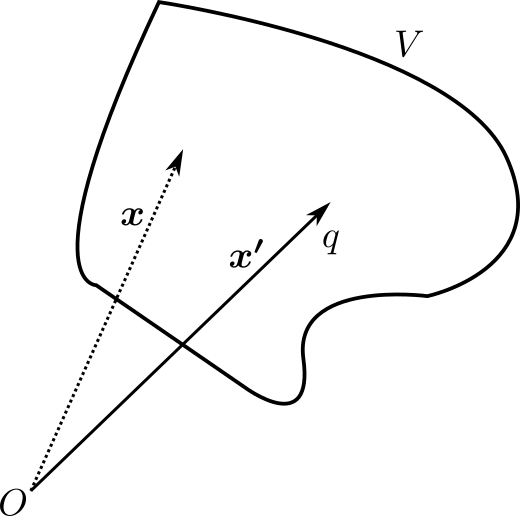
\includegraphics[width = 0.45\textwidth]{chargeinV.png}
    \caption{A volume $V$ contating a charge $q$.}
    \label{fig:chargeinV}
\end{figure}
Consider Gauss' law for a point charge sitting at $\vec{x'}$(Fig.~\ref{fig:chargeinV}). In some volume $V$, we have
\begin{equation*}
    \div \vec{E}(\vec{x'}) = \frac{q}{\varepsilon_0}\delta(\vec{x}-\vec{x'}).
\end{equation*}
Recall that for static charges,
\begin{equation*}
    \vec{E} = -\grad \Phi.
\end{equation*}
Thus, we arrive at the Possion's equation for a static charge
\begin{equation}
    \laplacian\Phi(\vec{x}) = -\frac{q}{\varepsilon_0}\delta(\vec{x} - \vec{x'}).
\end{equation}

Now, imposing the following boundary conditions
\begin{equation}
    \Phi(x) \to \phi_s \text{ as } \abs{\vec{x} - \vec{x'}} \to \infty. \label{eqn:bcFreespace}
\end{equation}
From the following realtionship (Note that $\curly{r} = \vec{x} - \vec{x'}$)
\begin{subequations}
    \begin{align}
        \div\left(\frac{\hat{\curly{r}}}{\curly{r}^2}\right) & = 4\pi\delta(\vec{\curly{r}})           \\
        \grad(\frac{1}{\abs{\curly{r}}})                     & = -\frac{\hat{\curly{r}}}{\curly{r}^2},
    \end{align}
\end{subequations}
we can establish the following
\begin{equation}
    \Phi(x) = q \underbrace{\frac{1}{4\pi\varepsilon_0}\frac{1}{\abs{\curly{r}}}}_{=G_0(\curly{r})} + \phi_s
\end{equation}
Here, $G_0$ is called the \textbf{free-space Green's function}. Free-space implies that $\Phi(\vec{x}) \to 0$ as $\curly{r} \to \infty$. In other words, $G_0$ is the solution of
\begin{equation}
    \laplacian G(\curly{r}) = -\frac{1}{\varepsilon_0} \delta(\curly{r}) \label{eqn:Gfn5}
\end{equation}
in the volume $V$, subject to the boundary condition (\ref{eqn:bcFreespace}) with $\phi_s = 0$.

Now, consider a collection of point charges $q_i$ at $\vec{x_i}$ where $\vec{x_i} \in V$ subject to the same boundary condition (\ref{eqn:bcFreespace}). Then by the principle of superposition
\begin{equation}
    \laplacian \Phi_{\text{total}}(\vec{x}) = \sum_{i = 1}^{N}\laplacian\Phi(\vec{x}) = - \sum_{i = 1}^{N} \frac{q_i}{\varepsilon_0} \delta(\curly{r}),
\end{equation}
and the solution is
\begin{subequations}
    \begin{align}
        \Phi_{\text{total}}(\vec{x}) = \sum_{i = 1}^{N} \Phi_i(\vec{x}) = \sum_{i = 1}^{N} q_i G_0 + \phi_s \\
        \implies \text{Continuum Limit} = \iiint_{V} \rho(\vec{x'}) G_0 + \phi_s \dmr{\vec{V}}.
    \end{align}
\end{subequations}
Thus, Green's function is essentially the linear response of the system at $\vec{x}$ to a point source at $\vec{x}$.


\subsection{The General Case}
The previous example is simple because the boundary conditions are trivial. In order to obtain the general Green's function solution for arbitrary boundary conditions, we need to use the first and second Green's identities.
\begin{subequations}
    \begin{align}
         & \iiint_{V}\left[\Phi\laplacian\Psi + \grad\Phi \cdot \grad\Psi\right] \dmr{\vec{V}} = \oiint_S (\Phi\grad\Psi)\cdot\dmr{\vec{S}} \label{eqn:G1ID}                          \\
         & \iiint_{V}\left[\Phi\laplacian\Psi - \Psi\laplacian\Phi\right] \dmr{\vec{V}} = \oiint_S \left[ \Phi\grad\Psi - \Psi\grad\Phi \right] \cdot \dmr{\vec{S}}; \label{eqn:G2ID}
    \end{align}
\end{subequations}
Where $\Phi$ and $\Psi$ are scalar functions, and the identities follow essentially from the divergence theorem.

Now, let $\Phi$ be the potential and $\Psi(\vec{x}) = G(\vec{x}, \vec{x'})$. Then the second identity (\ref{eqn:G2ID}) becomes
\begin{equation}
    \begin{split}
        \iiint_{V} \Phi(\vec{x'}) \nabla^{'2} G &\dmr{\vec{V}} \\
        &= \iiint_{V} G \nabla^{'2} \Phi(\vec{x'}) \dmr{\vec{V}} + \oiint_S \left[ \Phi(\vec{x'}) \grad' G - G\grad'\Phi(\vec{x'})  \right] \dmr{\vec{S}}. \label{eqn:Green9}
    \end{split}
\end{equation}
Now, using Eqn.~\ref{eqn:Gfn5}, we arrive at
\begin{equation}
    \iiint_{V} \Phi(\vec{x'}) \nabla^{'2} G \dmr{\vec{V}} = -\frac{1}{\varepsilon_0}\iiint_V \Phi(\vec{x'})\delta(\vec{x}-\vec{x'})\dmr{\vec{V}} = -\frac{1}{\varepsilon_0}\Phi(\vec{x}). \label{eqn:Green10}
\end{equation}
And, by Possion's equation $\laplacian\Phi = - \frac{\rho}{\varepsilon_0}$, we have
\begin{equation}
    \iiint_{V} G \nabla^{'2} \Phi(\vec{x'}) \dmr{\vec{V}} = -\frac{1}{\varepsilon_0}\iiint_V G(\vec{x},\vec{x'})\rho(\vec{x'})\dmr{\vec{V}}. \label{eqn:Green11}
\end{equation}
Thus, using Eqn.~\ref{eqn:Green10} \& Eqn.~\ref{eqn:Green11}, Eqn.~\ref{eqn:Green9} becomes
\begin{equation}
    \begin{split}
        \Phi(\vec{x}) = \iiint_V \rho(\vec{x'})G(\vec{x}, \vec{x'}) \dmr{\vec{V}} &- \varepsilon_0 \oiint_S\nabla'G(\vec{x}, \vec{x'})\Phi(\vec{x'})\cdot\dmr{\vec{S}}\\
        &+ \varepsilon_0\oiint_S\nabla'\Phi(\vec{x'})G(\vec{x}, \vec{x'})\cdot\dmr{\vec{S}}.
    \end{split}
\end{equation}
This is known as the solution for the \textbf{general Green's function}.
\end{document}